\documentclass[a4paper,14pt]{article}
\usepackage{blindtext}
\usepackage[T2A]{fontenc}
\usepackage[utf8]{inputenc}
\usepackage[english,russian]{babel}
\usepackage{listings}
\usepackage{geometry}
\usepackage{amssymb}
\usepackage{amsmath}
\usepackage[14pt]{extsizes}
\geometry{left=3cm}
\geometry{right=1.5cm}
\geometry{top=2cm}
\geometry{bottom=2cm}
\pagestyle{plain}
\usepackage{pgfplots}
\usepackage{filecontents}
\usepackage{graphicx}
\usepackage{indentfirst}
\DeclareGraphicsExtensions{.png}
\graphicspath{{images/}}
\usetikzlibrary{datavisualization}
\usetikzlibrary{datavisualization.formats.functions}
\usepackage{tabularx}
\pgfplotsset{width=7 cm}
\usepackage{xcolor}
%\renewcommand{\rmdefault}{ftm}
%\usepackage{mathptmx}
\usepackage{setspace}
%\usepackage{minted}
%\полуторный интервал
\onehalfspacing
\usepackage{colortbl}
\usepackage{tocloft}
\frenchspacing
\setcounter{page}{3}
\usepackage{multirow}
\usepackage{float}
\usepackage{multirow}

\renewcommand{\cftsecdotsep}{\cftdot}
\renewcommand{\cftsecleader}{\cftdotfill{\cftsecdotsep}}
\renewcommand{\cftsubsecleader}{\cftdotfill{\cftsecdotsep}}
\renewcommand{\cftsubsubsecleader}{\cftdotfill{\cftsecdotsep}}

%\renewcommand\cftchapdotsep{\cftdot}
%\renewcommand\cftsecdotsep{\cftdot}
%\renewcommand{\cftchapleader}{\cftdotfill{\cftchapdotsep}}

% Для измененных титулов глав:
% % подключаем нужные пакеты
%\definecolor{gray75}{gray}{0.75} % определяем цвет
%\newcommand{\hsp}{\hspace{20pt}} % длина линии в 20pt
% titleformat определяет стиль
%\titleformat{\chapter}[hang]{\Huge\bfseries}{\thechapter\hsp\textcolor{black}{|}\hsp}{0pt}{\Huge\bfseries}
%\usepackage{titlesec, blindtext, color}
%\titleformat{\chapter}[hang]{\Huge\bfseries}{\thechapter\hsp\textcolor{black}{|}\hsp}{0pt}{\Huge\bfseries}

% Для листинга кода:
\lstset{ %
extendedchars=\true,
inputencoding=utf8,
morekeywords={include, printf},
texcl=\true,
breaklines=\true,
escapeend=\end{russian},
escapechar=\%,
keepspaces=\true,
language=c,                 % выбор языка для подсветки
basicstyle=\small\sffamily, % размер и начертание шрифта для подсветки кода
numbers=left,               % где поставить нумерацию строк (слева\справа)
numberstyle=\tiny,           % размер шрифта для номеров строк
stepnumber=1,                   % размер шага между двумя номерами строк
numbersep=5pt,                % как далеко отстоят номера строк от подсвечиваемого кода
showspaces=\true,            % показывать или нет пробелы специальными отступами
showstringspaces=\true,      % показывать или нет пробелы в строках
showtabs=false,             % показывать или нет табуляцию в строках
frame=single,              % рисовать рамку вокруг кода
tabsize=4,                 % размер табуляции по умолчанию равен 2 пробелам
captionpos=t,              % позиция заголовка вверху [t] или внизу [b]
breaklines=true,           % автоматически переносить строки (да\нет)
breakatwhitespace=false, % переносить строки только если есть пробел
escapeinside={\//*}{*)}   % если нужно добавить комментарии в коде
}



\begin{document}

\begin{titlepage}

    \begin{table}
        \centering
        \footnotesize
        \begin{tabular}{cc}
            \multirow{8}{*}{
\includegraphics[scale=0.35]{bmstu.jpg}}
             &                                                                           \\
             &                                                                           \\
             & \textbf{Министерство науки и высшего образования Российской Федерации}    \\
             & \textbf{Федеральное государственное бюджетное образовательное учреждение} \\
             & \textbf{высшего образования}                                              \\
             & \textbf{<<Московский государственный технический}                         \\
             & \textbf{университет имени Н.Э. Баумана>>}                                 \\
             & \textbf{(МГТУ им. Н.Э. Баумана)}                                          \\
        \end{tabular}
    \end{table}

    \vspace{-2.5cm}

    \begin{flushleft}
        \rule[-1cm]{\textwidth}{3pt}
        \rule{\textwidth}{1pt}
    \end{flushleft}

    \begin{flushleft}
        ФАКУЛЬТЕТ Информатика и системы управления
    \end{flushleft}
    КАФЕДРА Программное обеспечение ЭВМ и информационные технологии

    \vspace{3cm}

    \begin{center}
        \textbf{Лабораторная работа № 8} \\
        \textbf{Дисциплина: <<Компьютерные сети>>}
        \vspace{0.5cm}
    \end{center}


    \vspace{3cm}

    \begin{flushleft}
        \begin{tabular}{ll}
            \textbf{Студент}       & Овчинникова А. П. \\
            \textbf{Группа}        & ИУ7-75Б           \\
            \textbf{Преподаватель} & Рогозин Н. О.     \\
        \end{tabular}
    \end{flushleft}

    \vspace{3cm}

    \begin{center}
        Москва, 2020 г.
    \end{center}

\end{titlepage}

\setcounter{page}{2}

\subsection*{Стенд 1}

На рисунках \ref{fig:pc1_set} - \ref{fig:pc1_set2} представлена настройка PC0.


\begin{figure}[!h]
    \center{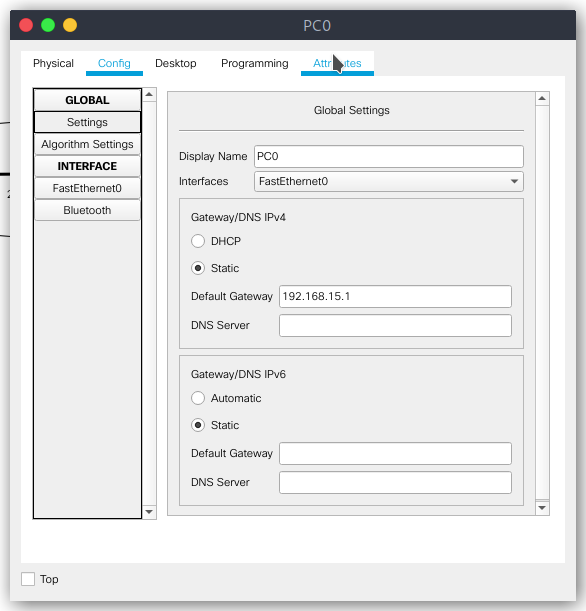
\includegraphics[width=14cm]{pc1_set}}
    \caption{Настройка PC0 (часть 1).}
    \label{fig:pc1_set}
\end{figure}

\newpage
\begin{figure}[!h]
    \center{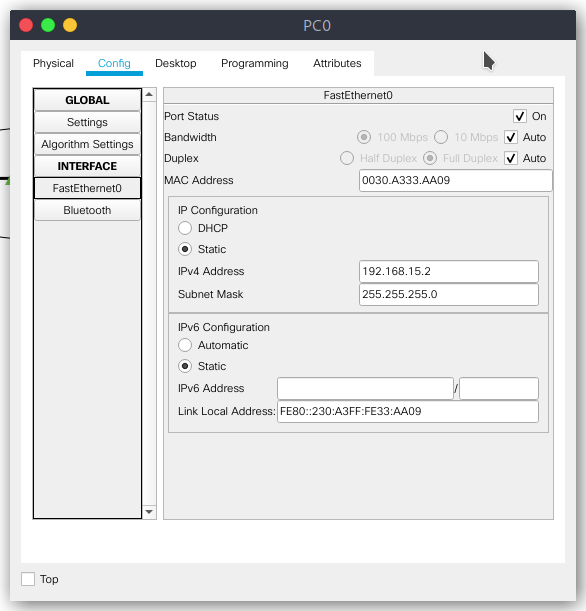
\includegraphics[width=14cm]{pc1_set2}}
    \caption{Настройка PC0 (часть 2).}
    \label{fig:pc1_set2}
\end{figure}

\newpage
На рисунках \ref{fig:r0_set} - \ref{fig:r0_set3} изображена настройка Router0.


\begin{figure}[!h]
    \center{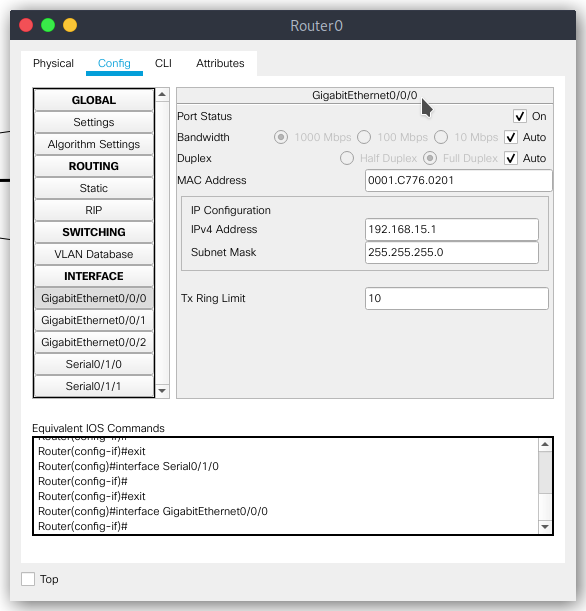
\includegraphics[width=14cm]{r0_set}}
    \caption{Настройка Router0 (часть 1).}
    \label{fig:r0_set}
\end{figure}

\newpage
\begin{figure}[!h]
    \center{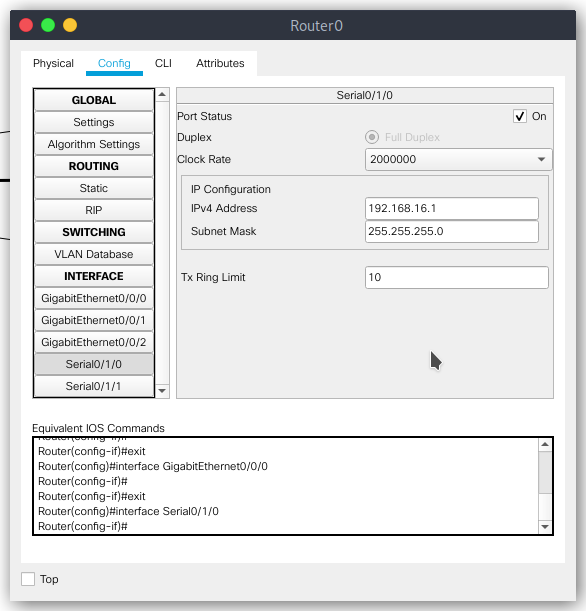
\includegraphics[width=14cm]{r0_set2}}
    \caption{Настройка Router0 (часть 2).}
    \label{fig:r0_set2}
\end{figure}

\newpage
\begin{figure}[!h]
    \center{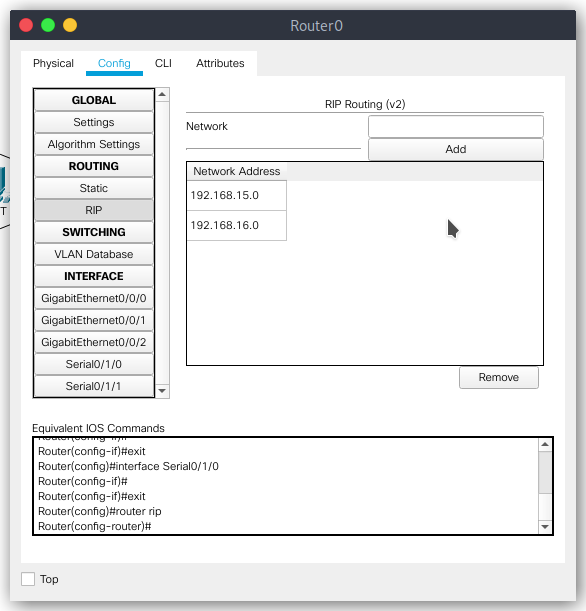
\includegraphics[width=14cm]{r0_set3}}
    \caption{Настройка Router0 (часть 3).}
    \label{fig:r0_set3}
\end{figure}

Последовательность команд для настройки Router0:

\textit{show ip protocols}

\textit{show ip rip database}

\textit{router rip}

\textit{network 192.168.15.0}

\textit{network 192.168.16.0}

\textit{version 2}

Настройка остальных роутеров и хостов производится аналогично. Таблица маршрутизации Router 1 приведена на рисунке \ref{fig:table}. Для каждого роутера должно быть две сети, к которым он подключен напрямую и две сети, к которым он подключается через другие маршрутизаторы.


\newpage
\begin{figure}[!h]
    \center{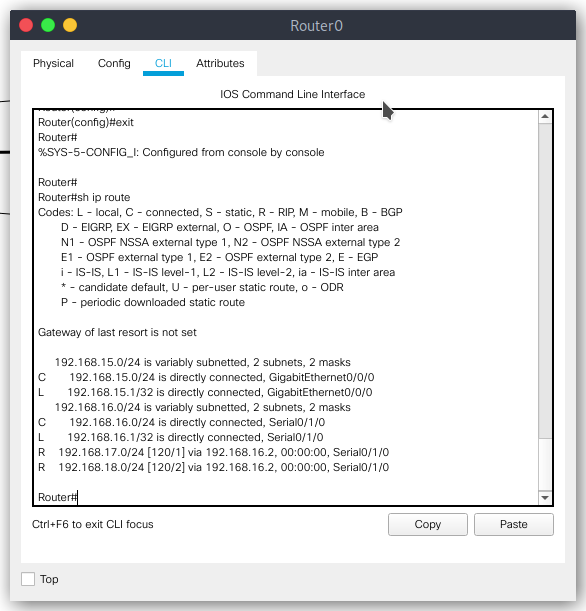
\includegraphics[width=14cm]{table}}
    \caption{Таблица маршрутизации Router 0.}
    \label{fig:table}
\end{figure}


Пример работы стенда 1 приведен на рисунках \ref{fig:ping1} - \ref{fig:ping2}.
\newpage
\begin{figure}[!h]
    \center{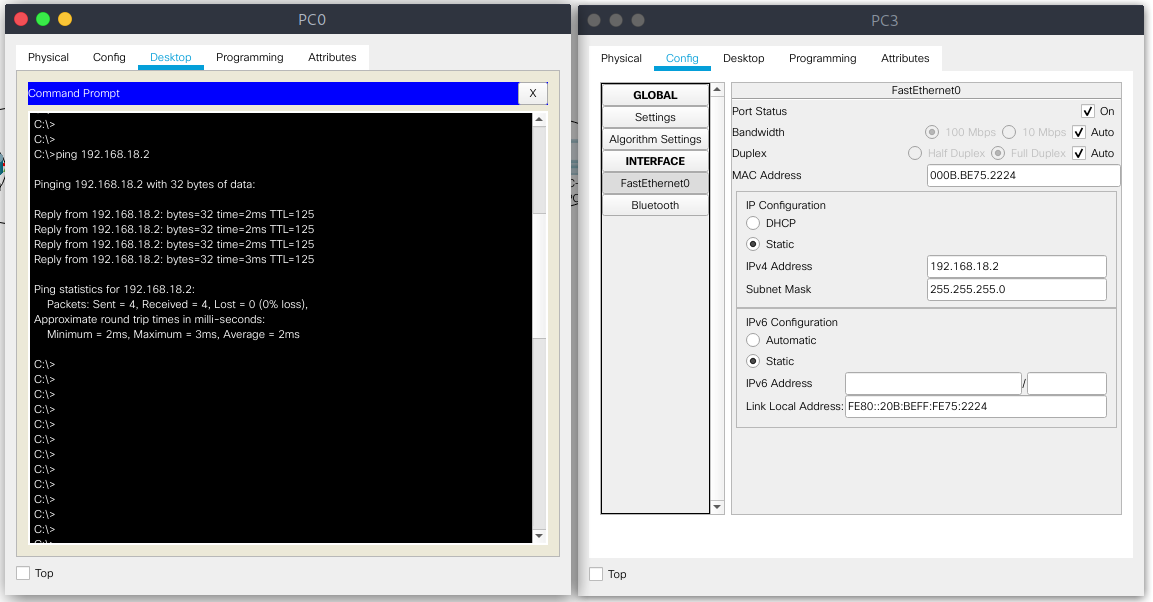
\includegraphics[width=16cm]{ping1}}
    \caption{Работа стенда.}
    \label{fig:ping1}
\end{figure}

\begin{figure}[!h]
    \center{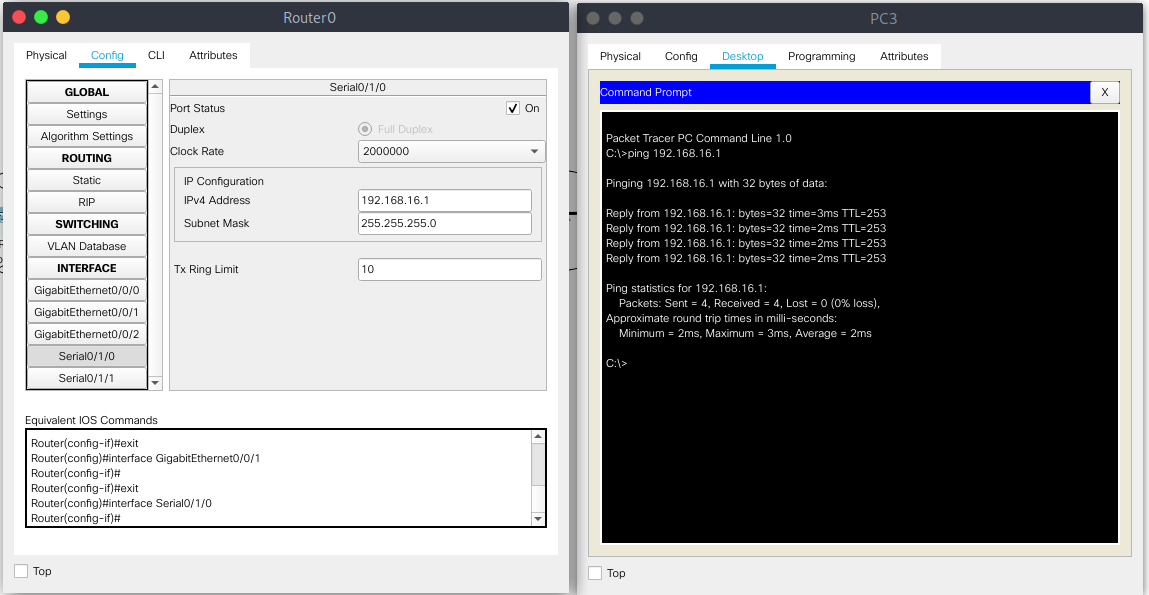
\includegraphics[width=16cm]{ping2}}
    \caption{Работа стенда.}
    \label{fig:ping2}
\end{figure}

\newpage
\subsection*{Стенд 2}

Пример настройки PC7 приведен на рисунках \ref{fig:pc7} - \ref{fig:pc7_2}.

\begin{figure}[!h]
    \center{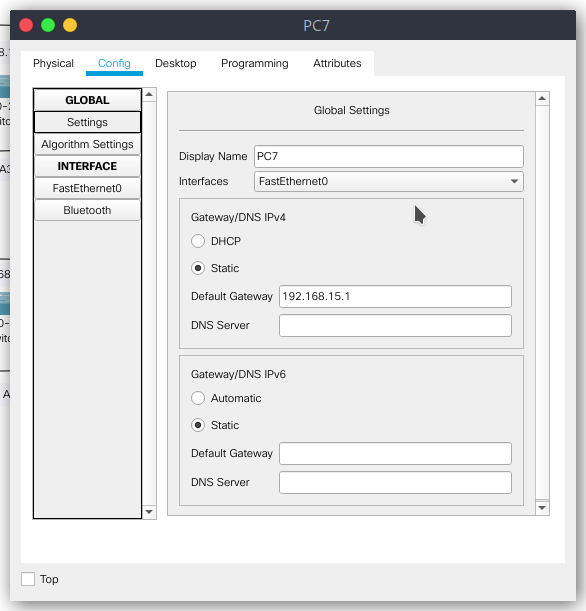
\includegraphics[width=14cm]{pc7}}
    \caption{Настройка PC7 (часть 1).}
    \label{fig:pc7}
\end{figure}
\newpage
\begin{figure}[!h]
    \center{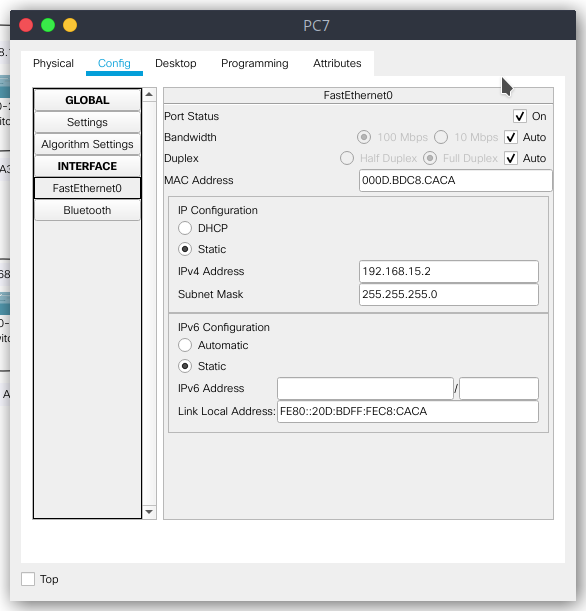
\includegraphics[width=14cm]{pc7_2}}
    \caption{Настройка PC7 (часть 2).}
    \label{fig:pc7_2}
\end{figure}

Пример настройки Router 7 приведен на рисунках \ref{fig:r7_1} - \ref{fig:r7_2}.

\newpage
\begin{figure}[!h]
    \center{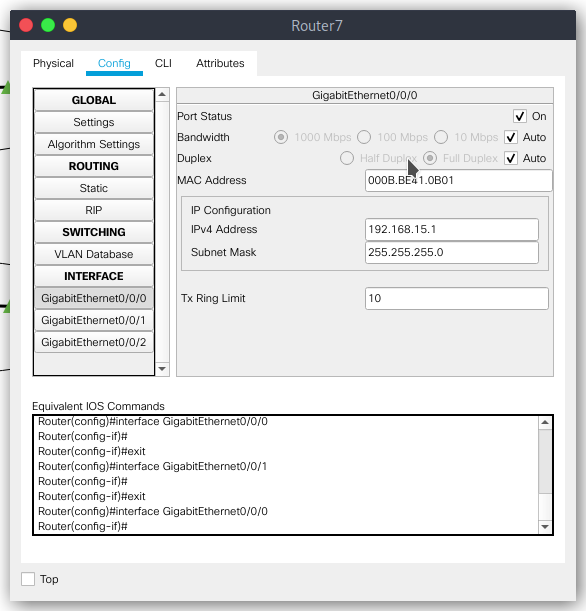
\includegraphics[width=14cm]{r7_1}}
    \caption{Настройка Router 7 (часть 1).}
    \label{fig:r7_1}
\end{figure}

\newpage
\begin{figure}[!h]
    \center{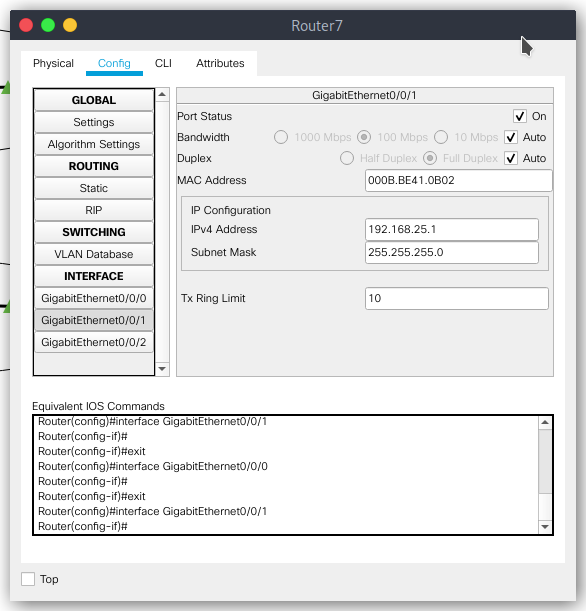
\includegraphics[width=14cm]{r7_2}}
    \caption{Настройка Router 7 (часть 2).}
    \label{fig:r7_2}
\end{figure}

Последовательность команд для настройки Router 7:

\textit{ip ospf authentication-key pass} (для GigabitEthernet 0/0/0)

\textit{ip ospf authentication-key pass} (для GigabitEthernet 0/0/1)

\textit{router ospf 1}

\textit{network 192.168.15.0 0.0.0.255 area 1}

\textit{network 192.168.25.0 0.0.0.255 area 0}

\textit{area 0 authentication}

\textit{area 1 authentication}

Настройка остальных хостов и маршрутизаторов производится аналогично.

На рисунке \ref{fig:r7_table} приведена таблица маршрутизации Router 7.

\newpage
\begin{figure}[!h]
    \center{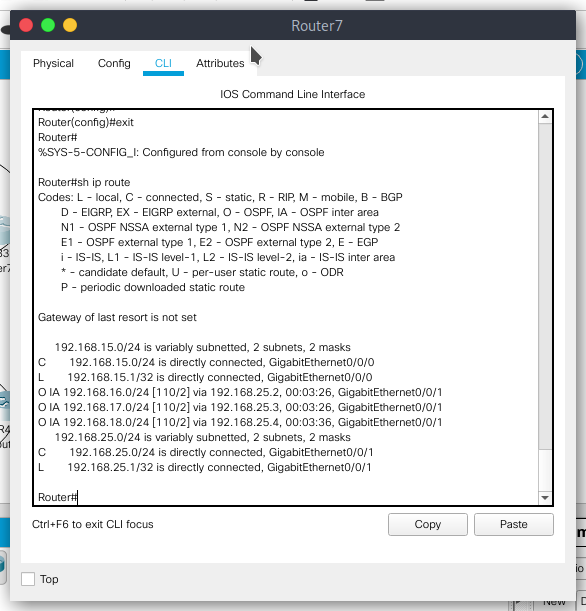
\includegraphics[width=14cm]{r7_table}}
    \caption{Таблица маршрутизации Router 7.}
    \label{fig:r7_table}
\end{figure}

\newpage
После настройки всех роутеров они видят соседей. На рисунке \ref{fig:r9_stat} приведена информация о статусе соседних устройств для Router 9.

\begin{figure}[!h]
    \center{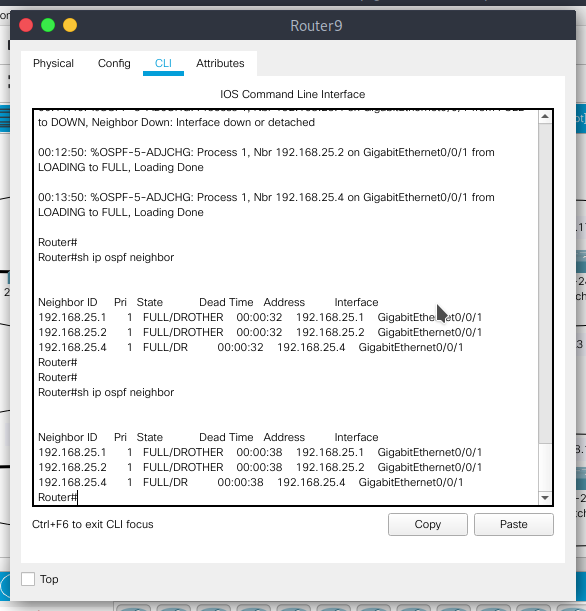
\includegraphics[width=14cm]{r9_stat}}
    \caption{Информация о статусе соседних устройств для Router 9.}
    \label{fig:r9_stat}
\end{figure}

\textbf{DR -- 192.168.25.4}

\textbf{BDR -- 192.168.25.3}

Примеры работы стенда 2 приведены на рисунках \ref{fig:pr3} - \ref{fig:pr4}.

\newpage
\begin{figure}[!h]
    \center{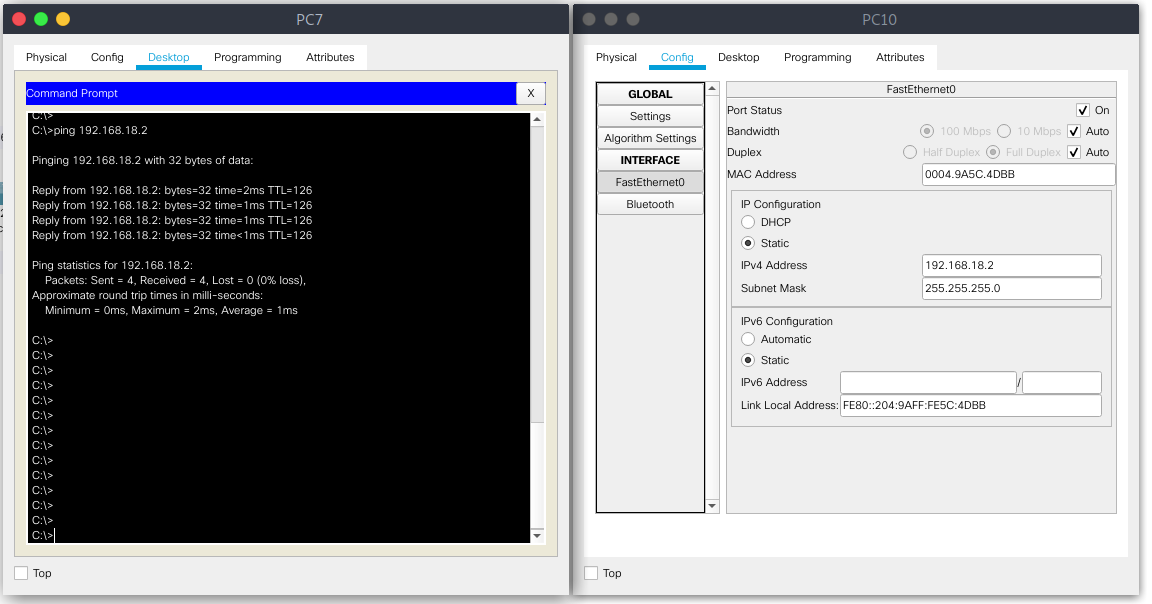
\includegraphics[width=16cm]{pr3}}
    \caption{Работа стенда.}
    \label{fig:pr3}
\end{figure}

\begin{figure}[!h]
    \center{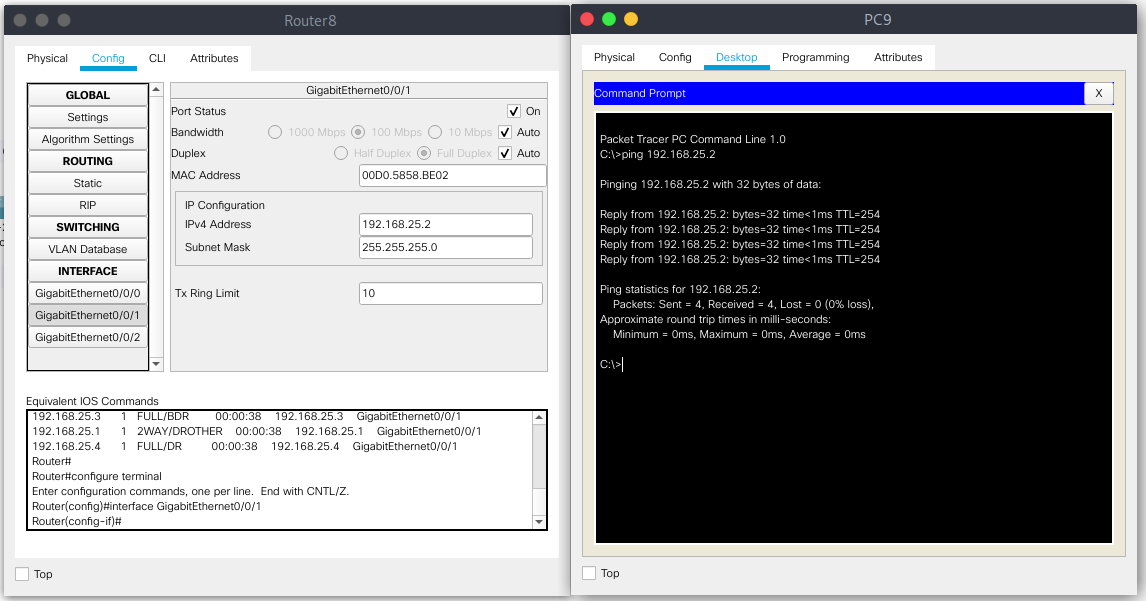
\includegraphics[width=16cm]{pr4}}
    \caption{Работа стенда.}
    \label{fig:pr4}
\end{figure}

\end{document}
